\chapter{Benutzerzentrierte Realisierung}\label{ch:benutzerzentrierte-realisierung} %TODO
Damit die Realisierung der graphisch-interaktiven Entwicklungsumgebung auf die Nutzenden angepasst werden kann, wurden die Vorlieben der Nutzenden mit verschiedenen Methoden abgefragt. Die daraus entstandenen Ergebnisse wurden bei der Entwicklung berücksichtigt. Das folgende Kapitel führt die beiden Konzepte ein und erklärt, wie diese angewendet wurden.

In Abschnitt \ref{sec:anforderungserhebung} wird das Konzept des Fragebogens erläutert, mit dem die Anforderungen der Nutzenden erhoben wurden. Daraufhin wird in Abschnitt \ref{sec:testsettings} die Struktur der teilnehmenden Beobachtung aufgeführt, mit der das Feedback der Nutzenden gesammelt wurde. Zuletzt wird in Abschnitt \ref{sec:operationalisierung} die Anwendung dieser beiden Konzepte und die Rekrutierung der Nutzenden dargelegt.

\section{Gestaltung der Anforderungserhebung}\label{sec:anforderungserhebung}
% Wie wurden anfänglich die Anforderungen der Nutzer erhoben?

Um die Entwicklungsumgebung auf die Bedürfnisse der Nutzenden anzupassen, müssen deren Anforderungen abgefragt werden. Zu diesem Zweck bietet sich besonders durch die Möglichkeit der Einbindung von zusätzlichen Medien eine gezielte Online-Befragung an \cite{Schnell2018MethodenES}. Aus den Ergebnissen dieser Befragung entstand dann ein anfänglicher Style-Guide für die Benutzeroberfläche.

Damit die Befragung nützliche Ergebnisse liefert, müssen alle Fragen verständlich, knapp und neutral formuliert sein \cite{Jacobsen2019PraxisbuchUuU}. Der Fragebogen wurde in einzelne Abschnitte unterteilt, die alle nötigen Informationen enthielten und ohne Scrollen angezeigt werden konnten. Um technischen Problemen, die durch verschiedene Endgeräte und Browser entstehen könnten \cite{Schnell2018MethodenES}, vorzubeugen, wurde die Online-Umfrage-Applikation LimeSurvey verwendet. Diese bot alle nötigen Funktionen wie die Möglichkeit, Teilnehmende an der Umfrage zu verwalten und die Daten in der Anwendung auszuwerten. %und wurde bereitgestellt? Zitieren?

Bevor den Teilnehmenden an der Umfrage Fragen gestellt wurden, wurde Pepper, siehe Kapitel \ref{ch:roboter-steuerung}, und das Anwendungsbeispiel in Abbildung \ref{fig:umfrage-anwendungsbeispiel} vorgestellt und erklärt. Das Anwendungsbeispiel, das die Umfrage begleitet, besteht nur daraus, dass Pepper sich vorstellt und dann das Gegenüber fragt, ob Pepper sich bewegen oder eine Geschichte erzählen soll. Sagt die Person "Bewegen" oder "Geschichte", führt Pepper die gewünschte Aktion aus.

\begin{figure}[t]
	\centering
	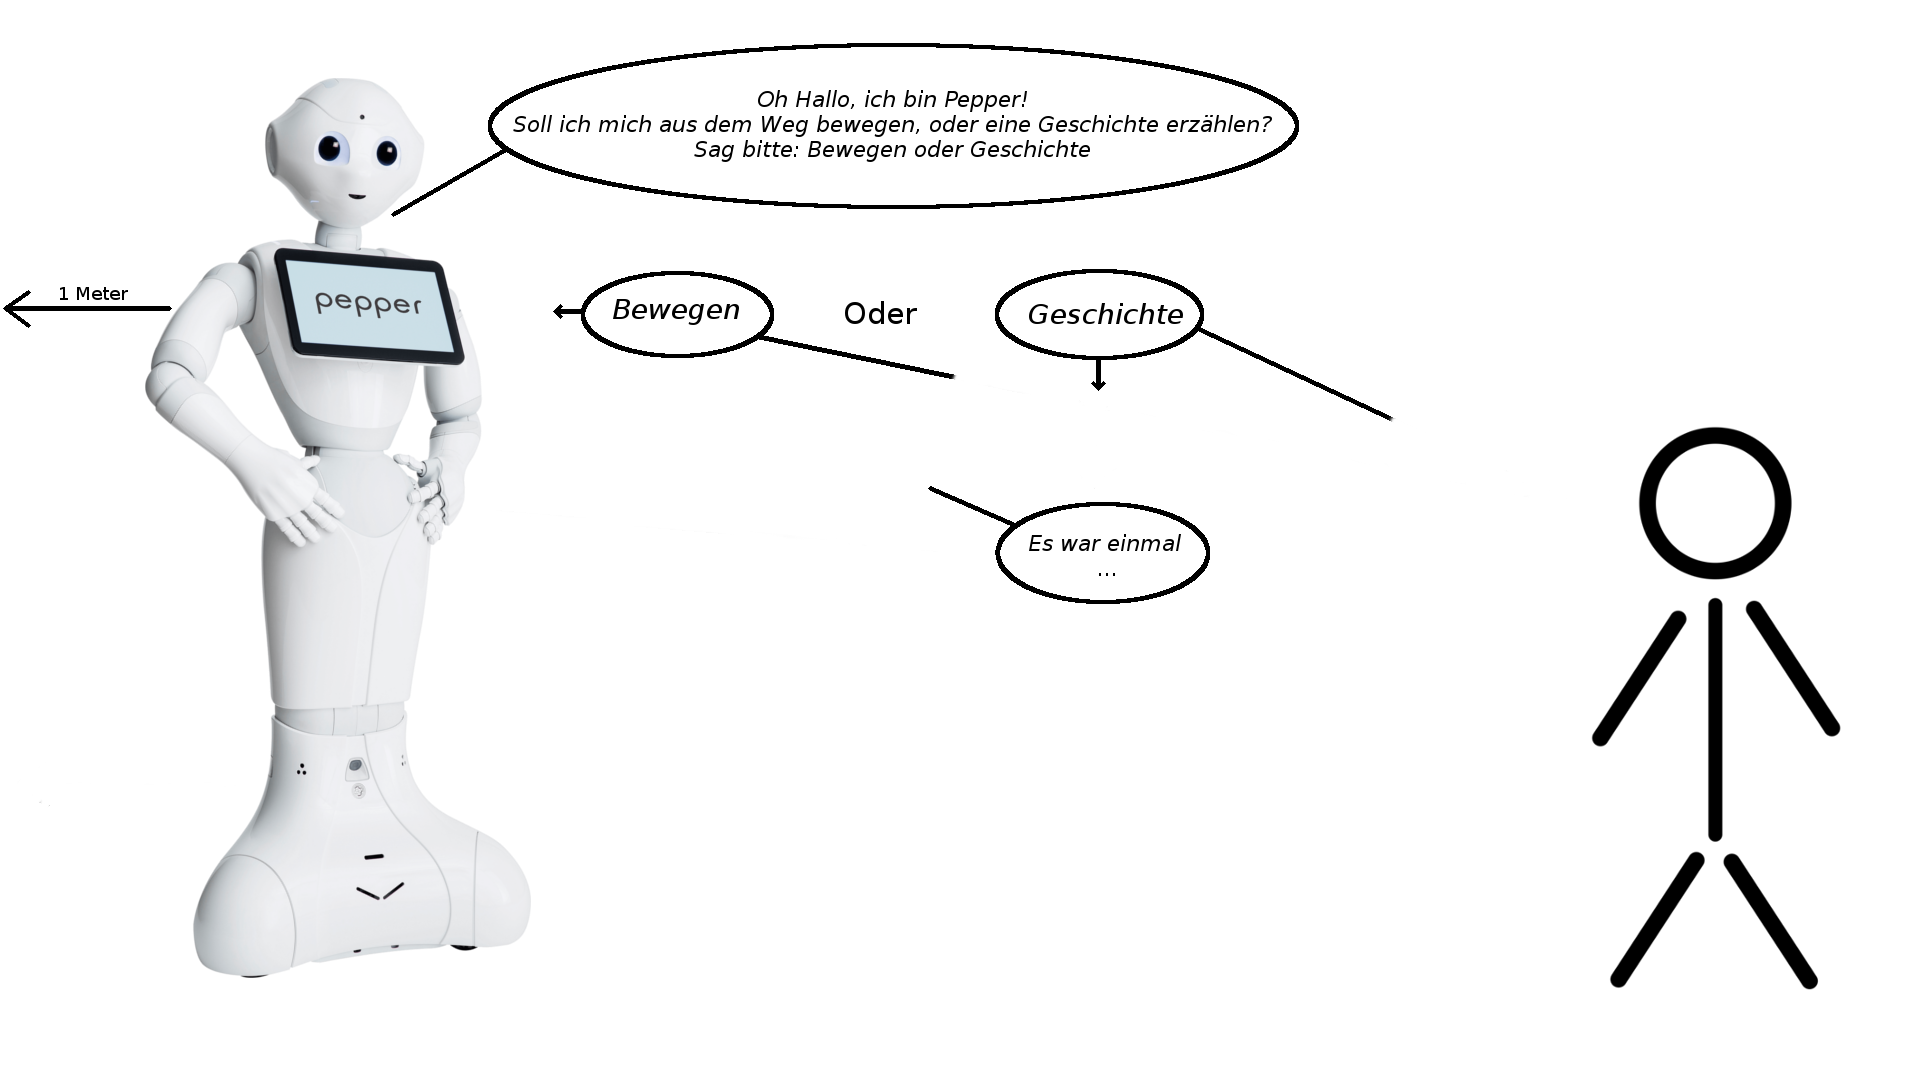
\includegraphics[width=13cm]{Plots/umfrage-anwendungsbeispiel.png}
	\caption{Anwendungsbeispiel der Anforderungserhebung.}
	\label{fig:umfrage-anwendungsbeispiel}
\end{figure}


In den folgenden Abschnitten werden die einzelnen Teile des Fragebogens und deren Nutzen für den Entwicklungsprozess aufgeführt. Die Auswertung der Ergebnisse des Fragebogens folgt in Kapitel \ref{sec:quanti-auswertung}.

\subsection{Vergleich mit bestehenden Anwendungen}
Der erste Anschnitt der Umfrage stellt Choregraphe, siehe Abschnitt \ref{sec:stand-der-technik}, und das Konzept der Entwicklungsumgebung mithilfe eines Mock-ups vor. Dabei werden die grundlegenden Funktionen beider Programme erläutert. Dazu wird jeweils die Realisierung des Anwendungsbeispiels aus Abbildung \ref{fig:umfrage-anwendungsbeispiel} in beiden Entwicklungsumgebungen, siehe Abbildung \ref{fig:umfrage-anwendung}, dargestellt.

\begin{figure}[t]
	\centering
	\begin{subfigure}{.5\textwidth}
		\centering
		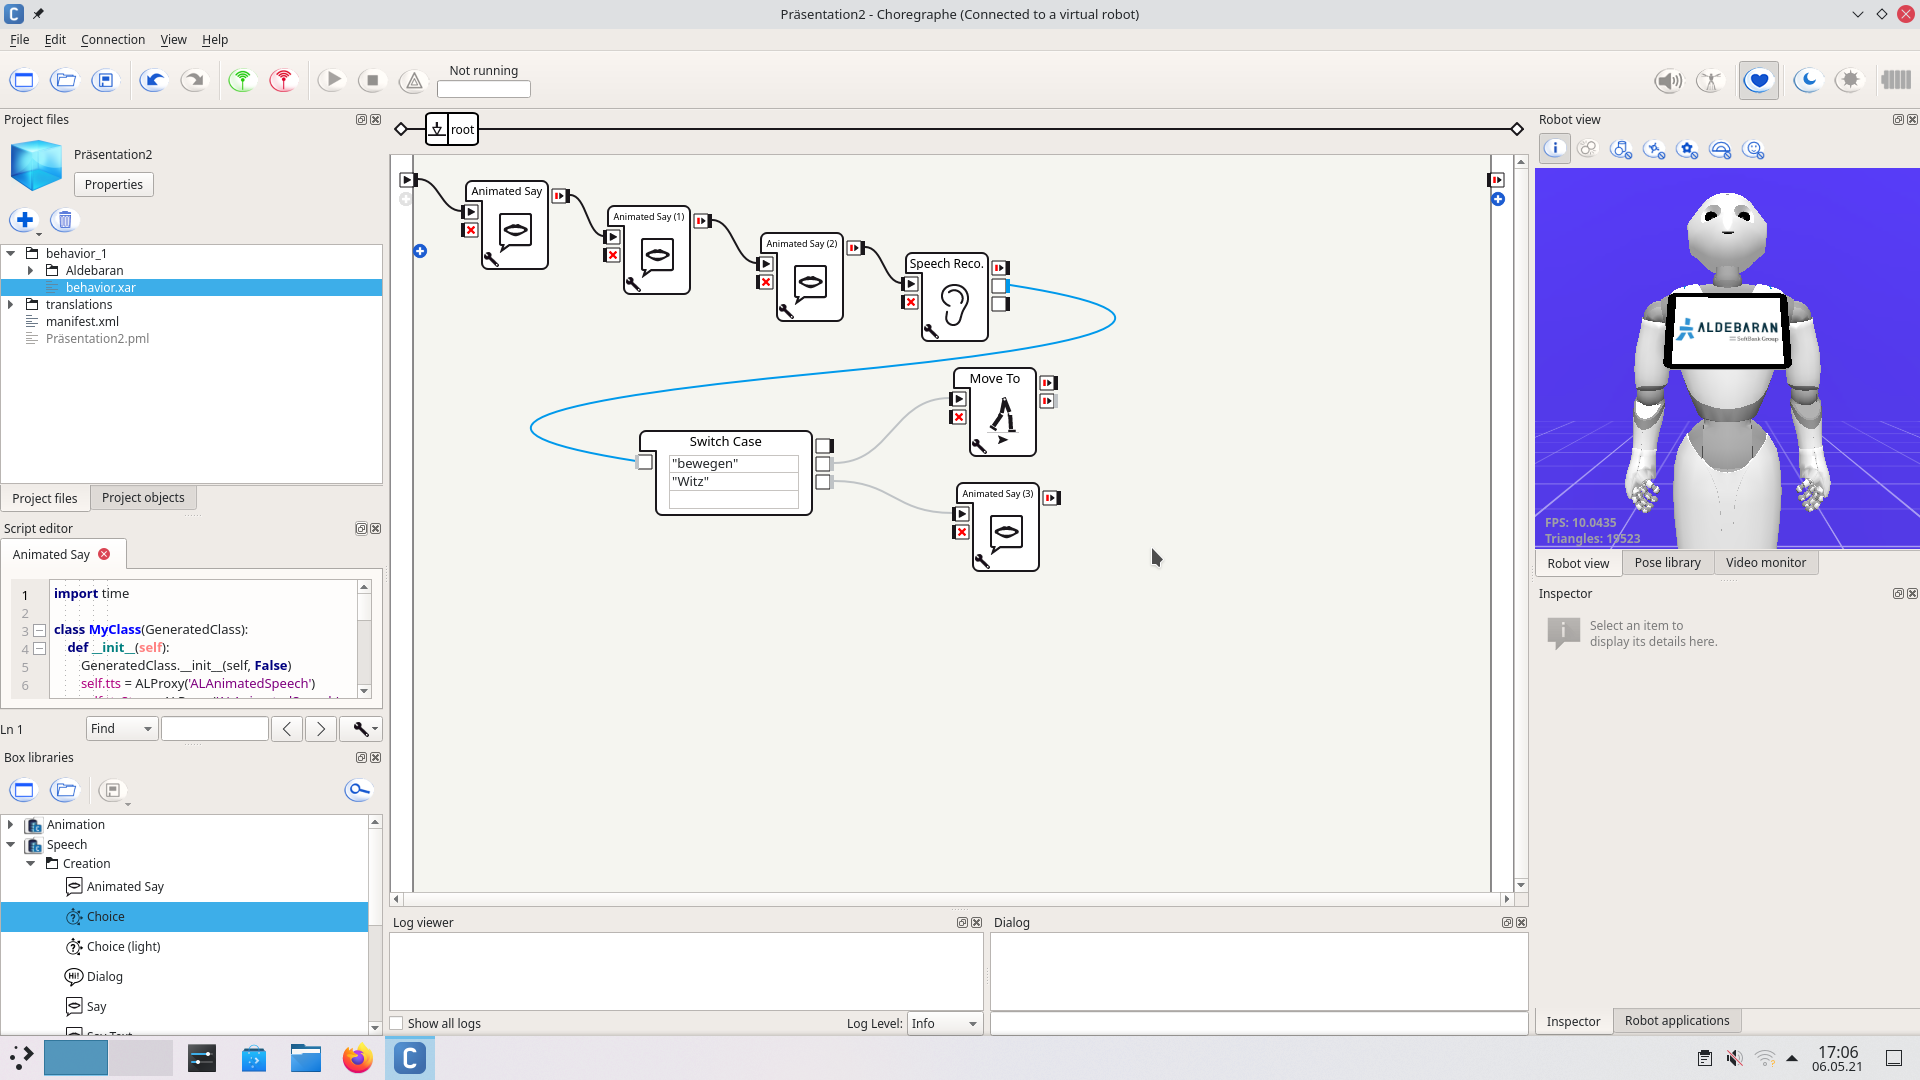
\includegraphics[width=\linewidth]{Plots/umfrage-choregraphe-anwendung.png}
		\caption{Anwendung in Choregraphe.}
		\label{subfig:choregraphe-anwendung}
	\end{subfigure}%
	\begin{subfigure}{.5\textwidth}
		\centering
		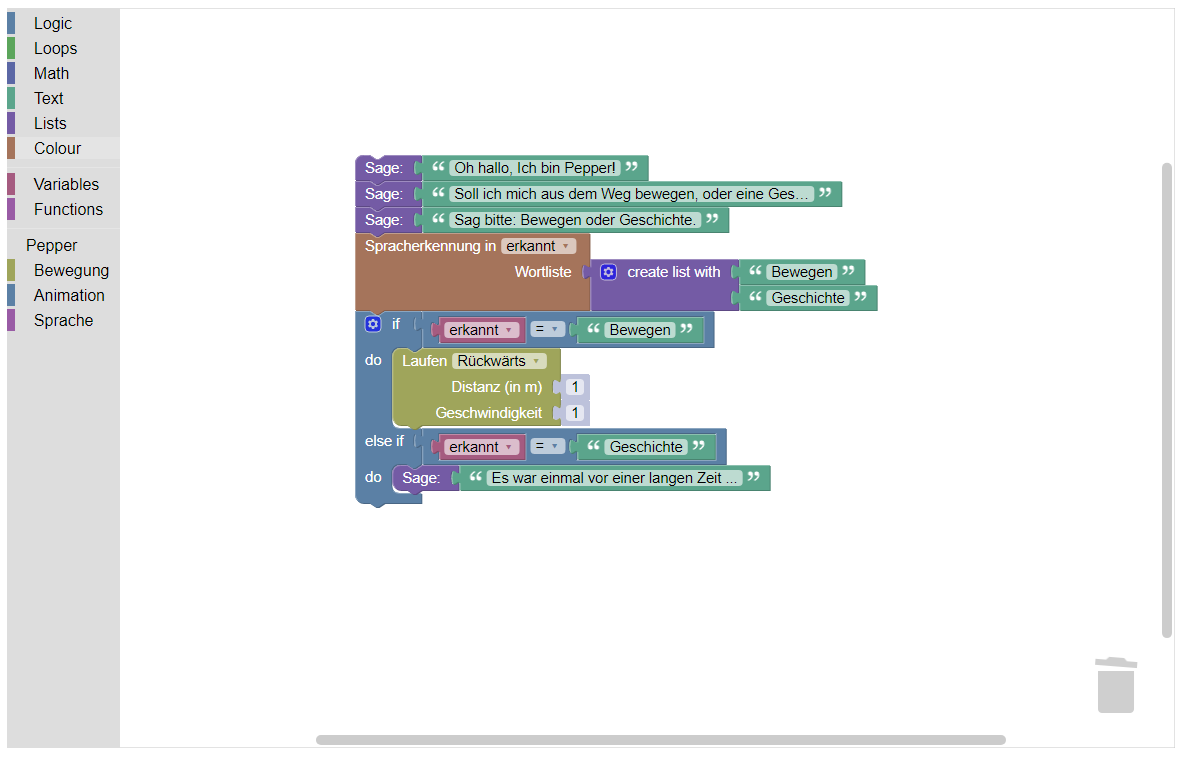
\includegraphics[width=\linewidth]{Plots/umfrage-blockly-anwendung.png}
		\caption{Anwendung im Blockly Mock-up.}
		\label{subfig:blockly-anwendung}
	\end{subfigure}
	\caption{Das Anwendungsbeispiel in Choregraphe und dem Blockly Mock-up umgesetzt.}
	\label{fig:umfrage-anwendung}
\end{figure}

Die Teilnehmenden an der Umfrage werden daraufhin aufgefordert, neun Aussagen auf je einer Skala für beide Entwicklungsumgebungen zu bewerten. Zu diesem Zweck wurde eine 5-Punkte Likert-Skala \cite{Schnell2018MethodenES} verwendet, die eine neutrale Antwortmöglichkeit zulässt. Diese sollte existieren, damit die Teilnehmenden nicht gezwungen sind, eine Entscheidung zu treffen \cite{Willits2016AnotherLookLikert}, falls sie wegen ihrer fehlenden Erfahrung unsicher sind. Die beiden Extrema der Skala sind mit "1: Stimme überhaupt nicht zu" und "5: Stimme voll zu" beschriftet. Diese Skala wird im weiteren Verlauf des Fragebogens weiterhin verwendet, um Konsistenz zu schaffen.

Die Aussagen beziehen sich insbesondere auf Verständlichkeit der Benutzeroberfläche, Einschätzung der eigenen Fähigkeit, die Entwicklungsumgebung zu nutzten und Interesse an der Nutzung der Anwendungen. %TODO Direkt die Aussagen hier einbinden? -> 121321311 (1 Verst., 2 Eisch., 3 Int.)

Die hier erhobenen Daten wurden dazu genutzt, eine erste Einschätzung des Mock-ups zu erlangen. Außerdem gaben sie eine Indikation, ob ein direkter Vergleich der beiden Entwicklungsumgebungen in den Nutzertests nötig ist.

\subsection{Blockgestaltung}
\colorbox{red}{Weiter, Übergänge dazwischen finden}

Wie bereits in Kapitel \ref{sec:visuelle-programmierung} dargelegt, gibt es verschiedene Möglichkeiten Blöcke in Blockly zu gestalten. Um diese Designentscheidungen den Nutzenden anzupassen, werden im zweiten Abschnitt der Online-Umfrage den Teilnehmenden jeweils verschiedene Mock-ups von funktional gleichen Blöcken präsentiert. Sie sollen dann den für sie am einfachsten verständlichen Block auswählen.

Die Auswahl der verschiedenen Optionen wurde so gewählt, dass die Mock-ups, die zur Auswahl stehen, jeweils Designentscheidungen repräsentieren. Beispielsweise steht die Entscheidung in Abbildung \textbf{TODO} repräsentativ für die Option einzelne Blöcke mit Hilfe von Drop-Down-Menüs zusammenzufassen und die Entscheidung Parameter-Slots generell extern (rechts) oder intern (mitten im Block) bereitzustellen. %TODO Zusammenschneiden der Designentscheidung 

Die gesammelten Antworten werden in den Style-Guide übersetzt, der die Vorlieben der Teilnehmenden an der Umfrage repräsentiert.

\subsection{Funktionale Anforderungen}
Im darauf folgenden Abschnitt des Fragebogens werden konkrete Anforderungen abgefragt. Den Teilnehmenden werden verschiedene Aussagen präsentiert, die sie auf einer 5-Punkte Likert-Skala bewerten sollen. Da die Teilnehmenden bereits eine Einführung in die Entwicklungsumgebung erhalten haben und sie im vorangegangenen Abschnitt des Fragebogens verschiedene Mock-ups und Kontrollelemente kennengelernt haben, haben sie nun ein Verständnis der Benutzeroberfläche um diese Anforderungen zu bewerten. %TODO etwas schöner formulieren?

Die abgefragten Anforderungen bezogen sich auf Barrierefreiheit, Sprache der Benutzeroberfläche, integrierte Funktionen in der Oberfläche, Benutzungsweise der Entwicklungsumgebung und weitere Funktionen dieser.

Teile dieser Anforderungen, wie die Sprache und Benutzungsweise der Benutzeroberfläche, flossen ebenso in den Style-Guide, siehe \ref{app:style-guide}, ein. Weitere Teile dieser Ergebnisse, wie etwa die Aussagen zu Barrierefreiheit, Erklärungen und Funktionen in der Benutzeroberfläche, bildeten eine Prioritäten-Liste von Funktionen, die in diese Anwendung eingefügt werden können.

%Eine weitere wichtige Komponente des Fragebogens ist die Abfrage der Anforderungen, die die Nutzer:innen an die Anwendung haben. Da diese inzwischen eine Einführung in die Entwicklungsumgebungen erhalten haben und in den Fragen zu den Designentscheidungen mit möglichen Mock-Ups der Kontrollelemente vertraut gemacht wurden, können sie hier einzelne Anforderungen einschätzen.
%
%Dies wird ebenfalls in Form von Aussagen umgesetzt, die die Teilnehmer:innen mit einer 5-Punkte Likert-Skala beantworten. Die Aussagen sind jeweils als technische Anforderungen formuliert, die Nutzer:innen von solchen Anwendungen an diese stellen könnten. Beispielsweise kann abgefragt werden, in welcher Sprache die Steuerelemente angezeigt werden sollten, welche weiteren Funktionen in der Oberfläche integriert werden sollten und welche Anforderungen an die Ausführung der Anwendung gestellt werden.
%
%Diese Ergebnisse werden dann teilweise, je nach Art der Aussage, in den Style-Guide oder eine Prioritäten-Liste der Anforderungen eingearbeitet, die die Wichtigkeit der Funktionen für die Prototypen und das endgültige Produkt angibt.

\subsection{Sonstige Datenerhebung}
Im abschließenden Teil der Umfrage wurden noch demographische Informationen, wie Studiengang und Semester, erfasst. Ebenso wurde die Programmier-Erfahrung der Teilnehmenden einfachen Ja-Nein-Fragen abgefragt.

Um Teilnehmende für die Nutzertests an den entstehenden Prototypen zu rekrutieren, wurden diese auf der letzten Seite der Online-Befragung dazu Aufgefordert eine E-Mail Adresse anzugeben. Da diese dann auch mit den Daten der vorangegangenen Fragen verknüpft sind, kann auch die Teilmenge der Nutzenden, die an den Nutzertests teilgenommen haben, in Kapitel \ref{sec:quanti-auswertung} einzeln betrachtet werden.

%In einem abschließenden Teil können noch Fragen gestellt werden, die Informationen über die Erfahrungen der Teilnehmer:innen mit Programmierung erheben. Ebenso können für die weiterlaufende Entwicklung relevante demographische Informationen abgefragt werden. Diese Abfrage kann in freier Form passieren.
%
%Um Teilnehmer:innen für die darauf folgenden Nutzertests an den entstehenden Prototypen zu rekrutieren werden diese auf der letzten Seite der Umfrage dazu aufgefordert bei Interesse ihre E-Mail Adresse anzugeben. Da diese dann auch mit den Daten der vorherigen Seiten verknüpft sind, kann später analysiert werden, ob die Teilnehmenden an den Nutzertests repräsentativ für die Befragten stehen.

\section{Instanziierung der Testsettings}\label{sec:testsettings} %TODO
Wie wurden die entstandenen Prototypen getestet? Welche Aufgaben sollten die Nutzer durchführen? Welche Involvierung hatte der Beobachter der Tests?

\section{Operationalisierung}\label{sec:operationalisierung}
Welche Nutzer? 